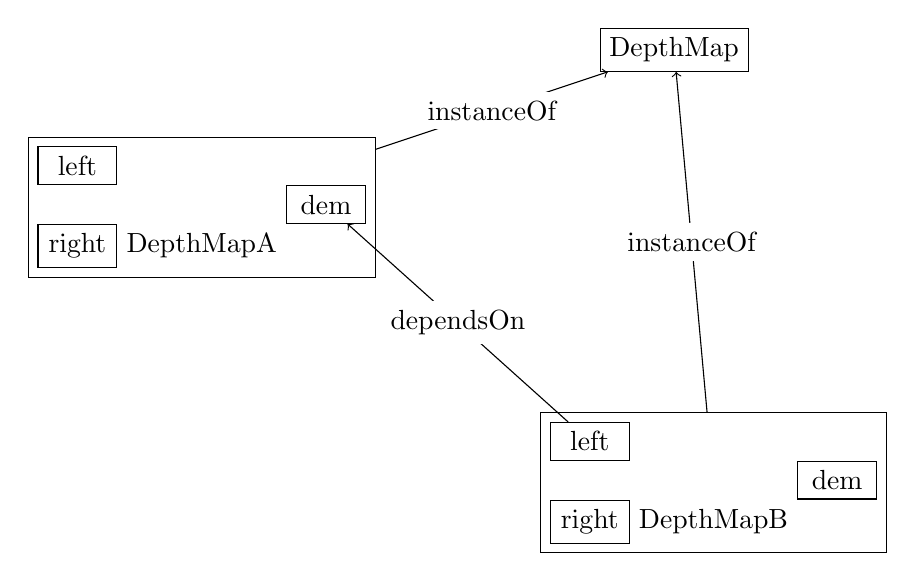
\begin{tikzpicture}[remember picture]
		\node[draw] (DepthMap) at (3,3) {
			DepthMap
		};
		\node[matrix, draw] (DepthMapA) at (-3,1) {
			\node[draw, minimum width=1cm] (left) {left}; & & \\
			& & \node[draw, minimum width=1cm] (demA) {dem}; \\
			\node[draw, minimum width=1cm] (right) {right}; & \node (label) {DepthMapA}; & \\
		};
		\node[matrix, draw] (DepthMapB) at (3.5,-2.5) {
			\node[draw, minimum width=1cm] (leftB) {left}; & & \\
			& & \node[draw, minimum width=1cm] (dem) {dem}; \\
			\node[draw, minimum width=1cm] (right) {right}; & \node (label) {DepthMapB}; & \\
		};
		\draw[->] (DepthMapA) to node[fill=white] {instanceOf} (DepthMap);
		\draw[->] (DepthMapB) to node[fill=white] {instanceOf} (DepthMap);
		\draw[->] (leftB) to node[fill=white] {dependsOn} (demA);
\end{tikzpicture}